% Drawing 138/07-2 -- folder 138, batch 07, archive page 122 (PDF page 123).
% Transcription: en marge gauche, un quadrilatère (enveloppe) dont les diagonales et deux segments se rencontrent en un point intérieur.
% Kind: quadrilateral (envelope) with diagonals. Method 2 (schematic redraw from the facsimile). Status: ok.
% Notes: Left margin: a quadrilateral drawn as an envelope (with a fifth corner at the left, as on the page), whose diagonals and two segments meet at an inner point; the right side is doubled.
% Coordinates: 1 unit = 1 mm = 1/100 of the crop width (bbox in page fractions: [0.136, 0.641, 0.25, 0.712]).
% Redrawn by Claude (claude-opus-5-5), issue #73, 2026-11-07; not checked by a human; not compiled (no TeX in the session).
% Rights: reproduces part of the work -- behind RENDER_TRANSCRIPTS, never published by itself.
\documentclass[tikz,border=3pt]{standalone}
\usepackage{amsmath,amssymb}
\usetikzlibrary{patterns,arrows.meta}
\tikzset{pencil/.style={black!45}, struck/.style={black!35}, mark/.style={circle,draw,inner sep=1.3pt}, pt/.style={circle,fill,inner sep=0.9pt}, opt/.style={circle,draw,fill=white,inner sep=1.1pt}}
\begin{document}
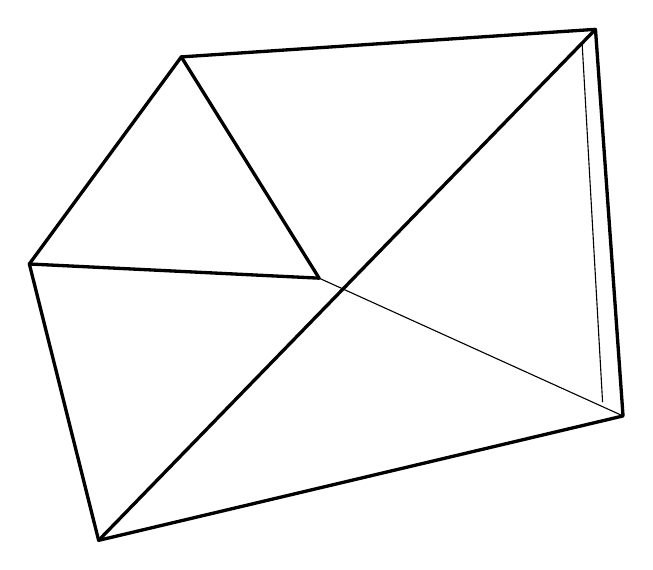
\begin{tikzpicture}[x=1mm,y=1mm,line cap=round,line join=round,font=\scriptsize]
\draw[very thick] (12.3,-42.1) -- (31.6,-15.8) -- (84.2,-12.3) -- (87.7,-61.4) -- (21.1,-77.2) -- cycle;
\draw (82.5,-14) -- (85.1,-59.6);
\draw[very thick] (31.6,-15.8) -- (49.1,-43.9);
\draw[very thick] (84.2,-12.3) -- (21.1,-77.2);
\draw[very thick] (12.3,-42.1) -- (49.1,-43.9);
\draw (49.1,-43.9) -- (87.7,-61.4);
\end{tikzpicture}
\end{document}
